\chapter{新算法的实验结果}
\label{cha:exp}

\section{IBM的测试数据集}

这一小节讲介绍测试数据集中关于供电网络的模型假设。

此数据集来源于IBM的公开数据~\cite{nassif2008power},在由IBM奥斯汀研究实验室举办的TAU 2011供电网络模拟竞赛中使用。 这个竞赛旨在寻找解决超大规模供电网络问题的有效方法。竞赛数据集的部分数据来源于真实的工业设计,另一部分
是对这些工业设计的扩展。这些数据能够帮助学术界的研究,并解决对超大规模供电网络分析日益增长的需求。对于参赛队伍的解决方案,主要从解(网络节点的电压降值)的精确度、运行时间、使用内存这三个方面去评价。
具体来说:精确度方面,最大的绝对误差不能超过10毫伏,平均绝对误差不能超过1毫伏;运行时间方面,在竞赛中将以一个Matlab标准解法作为比对,以参队队伍提出的算法的运行时间除以Matlab程序的运行时间作为参考;
内存方面,同样地将与之和Matlab程序使用的内存比较(这里的内存是指程序运行时间的最大使用内存量)。


此数据集共有六个电路参考设计,分别命名为IBMPG1到IBMPG6。表格\ref{tab:tabibm}总结了这几个设计的重要特征参数,包括电路的节点数、包含的纯电阻个数、包含的电压源与电流源个数、
金属层数等。整个数据集的节点数量之间的差距在两个数量级之间。

\begin{table}[htbp]
\centering
\caption{IBM供电网络测试集合}
\label{tab:tabibm}
\begin{tabular}{|c|r|r|r|r|r|r|}
\toprule[1.5pt]
\hline
数据编号 & 电流源数量 & 节点数量 & 电阻数量 & 短路数量 & 电压源数量 & 金属层数 \\
\hline
IBMPG1 & 10774 & 30638  & 30027  & 14208  &  14308 & 2\\
\hline
IBMPG2 & 37926 & 127238 & 208325 & 1298  & 330 & 5\\
\hline
IBMPG3 & 201054 & 851583 & 1401572 & 461 & 955 &  5\\
\hline
IBMPG4 & 276976 & 953583 & 1560645 & 11682 & 962  & 6\\
\hline
IBMPG5 & 540800 & 1079310 & 1076848 & 606587 & 539087 &  3\\
\hline
IBMPG6 & 761484 & 1670494 & 1649002 & 836107 & 936239 &  3\\
\hline
\end{tabular}
\end{table}

数据集文件用SPICE格式存储。具体的格式说明如下:

\begin{itemize}
\item 如果一行以星号(*)开头,那么这一行是注释;
\item 每一层电路的数据开头有一行注释:\emph{layer: <层名>,<网层> net: <网层序号>},例如\emph{layer: M1,Vdd net: 1}与\emph{layer: M1,Vss net: 2};
\item 层与层之间的连接(vias)数据前面会有一行注释:\emph{vias from: <网层序号> to <网层序号>};
\item 电路的节点形式为:\emph{n<网格序号>\_<节点x坐标>\_<节点y坐标>},例如"n3\_124\_921";
\item 如果一行的第一个字母是R,那么这一行的格式形如"Rxxxx Node1 Node2 value",其中“xxxx”是该电阻的名字(没有实际作用。可以忽略),表示Node1与Node2之间
有一个阻值为value的电阻;
\item 如果一行的第一个字母是V,那么这一行的格式形如"Vxxxx Node1 Node2 value",其中“xxxx”是该vias的名字(没有实际作用。可以忽略),表示Node1与Node2之间
有一个阻值为value的vias;value的值可以为0,表示这两个节点被短路了(通常用在两层之间相同位置的节点上);
\item 如果一行的第一个字母是r,那么这一行的格式形如"rxxxx Node1 Node2 value",其中“xxxx”是该电阻的名字(没有实际作用。可以忽略),表示Node1与Node2之间
有一个阻值为value的电阻;小写字母r开头的电阻与大写字母R的电阻的不同之处在于,小写字母r表示的是节点Node1和某个package(也就是Node2)(?)之间的电阻;例如Node1
如果名字是"n3\_123\_456",那么Node2一定是"\_X\_n3\_123\_456",所以这一行的形式为"rxxxx n3\_123\_456 \_X\_n3\_123\_456"。特殊的,电路数据文件里会指定这个package
的电压值,形式为"vxxxx Node2 0 value"其中Node2为小写字母r开头的数据中指定的package,value为该Node2的电压值;
\item 最后,负载电流源的形式为"iBxxxx Node 0 value"或者"iBxxxx 0 Node value“;分别表示从节点到Vdd的电流源大小或者从Vss到节点的电流大小。
\end{itemize}

\begin{figure}[H]
  \centering
  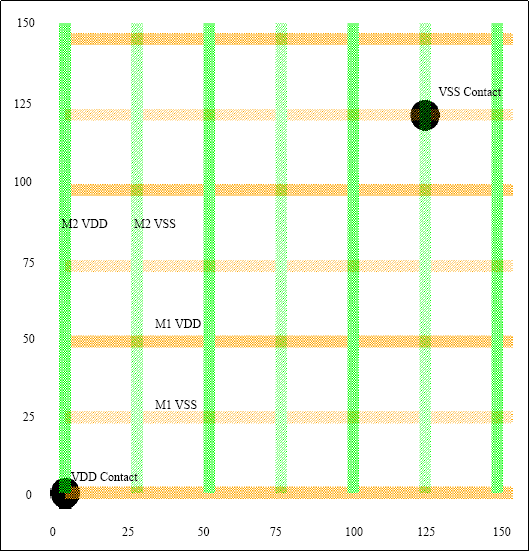
\includegraphics[height=8cm]{sample1}
  \caption{IBM供电网络测试数据集的数据样例~\cite{nassif2008power}}
  \label{fig:figsample1}
\end{figure}

图\ref{fig:figsample1}是一个比较小的供电网络例子。这个例子总共有两层金属网格,分别是水平排列的M1和垂直排列的M2;每一层金属网格都有4个Vdd线路和3个Vss线路;此供电网络
有两个package(用黑色实心圆圈表示),一个接电源,另一个接地。它的具体数据见附录B。使用第三节中的直接求解法,可以得到每个节点的对应电压降值。根据求出的电压降值,对
$V_{DD}$与$V_{SS}$分别绘制热度图可以得到图\ref{fig:figsample1-sol}。

\begin{figure}[H]
  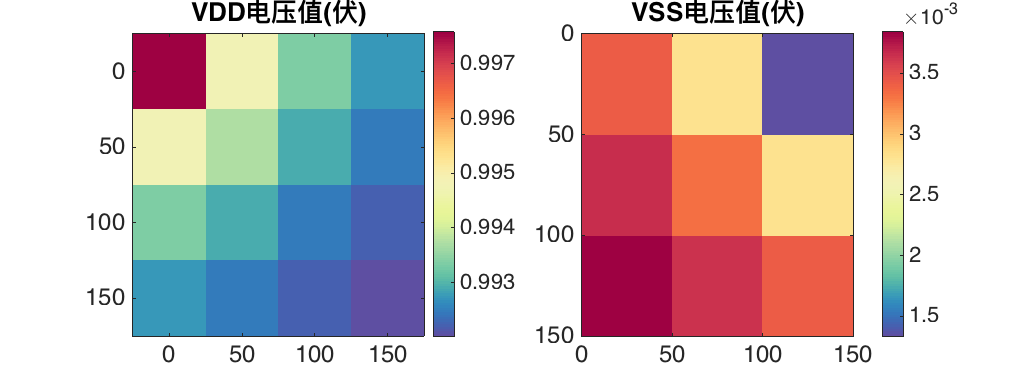
\includegraphics[height=6cm]{sample1-sol}
  \caption{样例数据的电压热度图}
  \label{fig:figsample1-sol}
\end{figure}

\section{实验平台}

实验使用的集群由8个节点组成,每个节点是一个Xeon E5-2699v4。Xeon E5-2699v4属于Intel Xeon®系列的处理器,有22个核心,基础频率是
2.20GHz,最高可超频至3.60GHz;并有55MB的智慧缓存(Smart Cache),支持DDR4 SDRAM内存。节点之间用Enhanced Data Rate(EDR)的Infiniband连接着,
EDR的传输速率可以达到100Gb/s。每一个节点有128GB的内存。

\section{预条件子算法与并行化的实验结果分析}

本文使用C++语言实现第三章中的算法,编译器是Intel CC 17.0.4,MPI库使用的是Intel MPI 2017.3.196。

程序时间的测量使用的是系统时钟,运行时间没有包括数据读入和输出的时间。在正确性校验中,比较的标准是计算出来的电压值不能与标准值(由IBM测试集提供)差距超过$10^{-3}$,
也就是1毫伏。

对于每个测试点,我们分别用1个、2个、4个、8个计算节点(核心)对其进行多进程测试,以此来考察并行化对算法的加速效果。使用不同数量的计算节点对程序运行效率的影响
如图\ref{fig:runtime}。正确性方面,由于数据集中已经提供了每个节点的实际电压降值,所以在实验中可以直接把算法求得的电压降值与解答文件中的值进行对比。对比的标准是
最大的电压降绝对误差不超过$0.1$毫伏。本实验的程序能够满足这个标准。

\begin{figure}[H]
  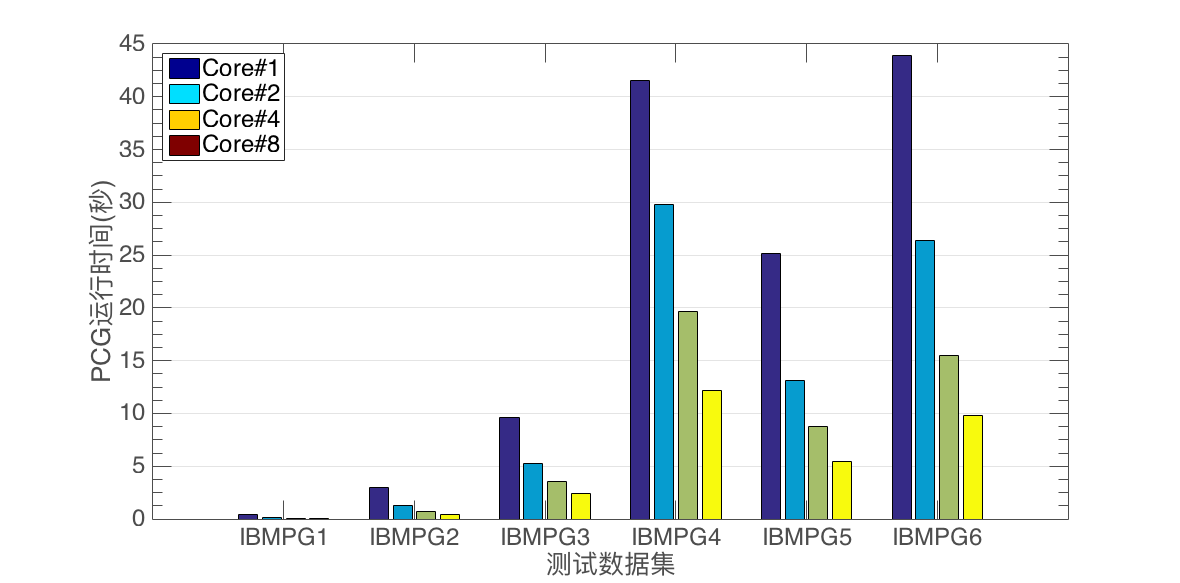
\includegraphics[height=8cm]{runtime}
  \caption{计算节点数目与运行时间的关系}
  \label{fig:runtime}
\end{figure}

\begin{sidewaystable}[htbp]
\centering
\caption{IBM数据集的测试结果}
\label{tab:tabibmresult}
\begin{tabular}{c|r|r|r|r|r|r|r|r}
\toprule[1.5pt]
\hline
数据编号 & 节点数量 & \textbf{计算节点数} & 迭代次数 & 通讯总量 & 非零元数量 & \makecell{通讯总量\\/非零元数量} & 运算时间(秒)
& \makecell{ \textbf{加速比} \\ \textbf{(相比单个运算节点)} } \\
\hline
IBMPG1 & 16327  & 1 & 172   &  0 & 75827 & 0\% & 0.427 & 1.000\\
\hline
& & 2 & 238 & 3438 & 75827 & 4.53\% & 0.119 & 3.602 \\
\hline
& & 4 & 254 & 6810 & 75827 &  8.98\% &  0.068 & 6.304 \\
\hline
& & 8 & 261 & 11208 & 75827 & 14.78\% & 0.081 & 5.265 \\
\hline
IBMPG2 & 126905 & 1 & 244 & 0 & 542895 & 0\% & 3.003 & 1.000 \\
\hline
& & 2 & 394 & 163410 & 542895 & 30.01\% & 1.291 & 2.325 \\
\hline
& & 4 & 405 & 172544 & 542895 & 31.78\% &  0.700 & 4.290 \\
\hline
& & 8 & 488 & 185346 & 542895 & 34.13\% & 0.459 & 6.543 \\
\hline
IBMPG3 & 285344 & 1 & 271 & 0 & 1508802 & 0\% & 9.663 & 1.000 \\
\hline
& & 2 & 412 & 18660 & 1508802 & 1.23\% & 5.241 & 1.844 \\
\hline
& & 4 & 471 & 262662 & 1508802 & 17.41\% & 3.600 & 2.685 \\
\hline
& & 8 & 510 & 319344 & 1508802 & 21.17\% & 2.447 & 3.948 \\
\hline
IBMPG4 & 952618 & 1 & 337 & 0 & 4054056 & 0\% & 41.532 & 1.000 \\
\hline
& & 2 & 563 & 1273824 & 4054056 & 31.421\% & 29.840 & 1.392 \\
\hline
& & 4 & 576 & 2136810 & 4054056 & 52.71\% & 19.695 & 2.101 \\
\hline
& & 8 & 568 & 2250576 & 4054056 & 55.51\% & 12.198 & 3.405 \\
\hline
IBMPG5 & 540220 & 1 & 336 & 0 & 2691958 & 0\% & 25.119 & 1.000 \\
\hline
& & 2 & 466 & 116832 & 2691958 & 4.34\% & 13.088 & 1.919 \\
\hline
& & 4 & 528 & 155100 & 2691958 & 5.76\% & 8.757 & 2.869 \\
\hline
& & 8 & 523 & 177632 & 2691958 & 6.60\% & 5.459 & 4.601 \\
\hline
IBMPG6 & 834252 & 1 & 390 & 0 & 4125504 & 0\% & 43.936 & 1.000 \\
\hline
& & 2 & 582 & 11148 & 4125504 & 0.27\% & 26.389 & 1.665 \\
\hline
& & 4 & 571 & 227452 & 4125504 & 5.51\% & 15.453 & 2.843 \\
\hline
& & 8 & 558 & 339142 & 4125504 & 8.22\% & 9.834 & 4.468 \\
\hline
\end{tabular}
\end{sidewaystable}

如果一个并行化算法是理想的,即忽略通讯交换数据带来的开销以及数据依赖带来的阻塞问题,那么算法的执行效率应该随着核心数的增加而线性增加,如图\ref{fig:figspeedupratio}
中的黑色虚线所示(其中,加速比的定义是串行算法的运行时间除以并行算法的运行时间;在本实验中,串行算法就是只有1个计算节点的情况,即单机执行;并行算法就是使用
多个计算节点的情况)。图\ref{fig:figspeedupratio}比较了理想情况下的加速比与实验中的加速比,可以看出,对于每个测试点,随着进程数/核心数的增加,
运行的时间是近线性地减少的。唯一的例外是IBMPG1对应的蓝色曲线,有一个拐点。这是因为IBMPG1的数据规模比较小,程序运行时间较短,所以并行化的效果并不显著。

需要注意的是,在使用不同数量的计算节点的时候,共轭梯度算法的迭代次数变化非常小,因此可以得出:在运算总次数极不不变的情况下,处理运算的运行效率提升了,
也就是说执行各种矩阵向量计算的效率也提升了。这证明了并行化算法的有效性。

此外,根据表格\ref{tab:tabibmresult},随着进程数/核心数的增加,通讯的代价也在增长,这主要体现在计算SPVM与向量内积时的数据通信上。当有多个计算节点时,一个节点
需要从系数矩阵中对应行涉及的列所在的节点中接受那些节点本地保存着的变量值;由于系数矩阵的对称性,这个节点也要发送本地的变量值给那些节点。具体来说,如果系数矩阵$A$的
第$i$行第$j$列不为0,即$A_{i,j}\neq 0$,并且行$i$与行$j$保存在不同的计算节点上时,这两个节点就要互相发送、接受$x_i$与$x_j$。
对于本算法来说,通讯的花销可以通过计算这样的$A_{i,j}$的数量来实现。这样的$A_{i,j}$越多,意味着在单次SPVM运算中节点间的通讯量越大。

图\ref{fig:figcomm}中有计算节点数与通讯量的关系图。为了让通讯量在电路节点数不同的数据之间可以比较,可以使用(系数矩阵中的跨节点的非零元$/$系数矩阵非零元)来表示相对通讯量的大小。
总的来说,通讯的花销阻碍了程序效率的进一步提升,导致算法的加速比没有达到理想的情况。在IBMPG6的测试中,使用了八个计算节点的并行化算法,相比单机算法只有4.468的加速比。

\begin{figure}[H]
  \centering
  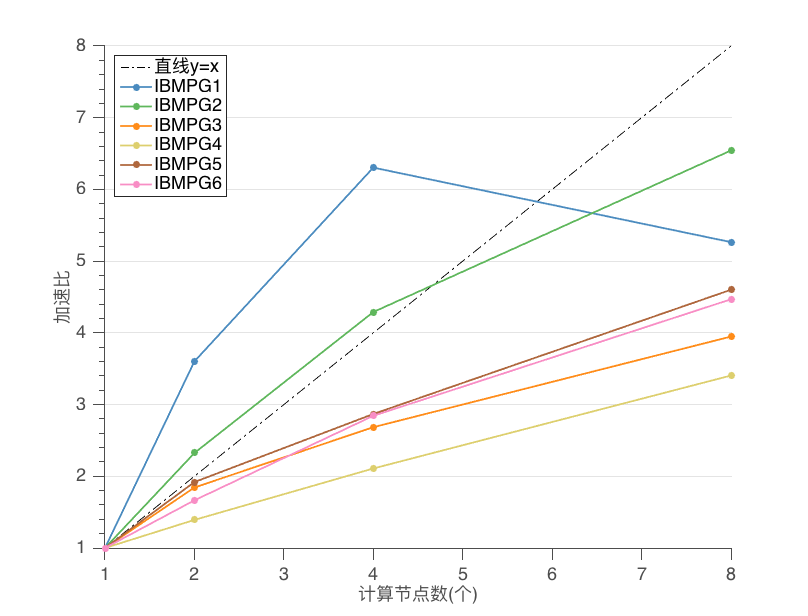
\includegraphics[height=10cm]{speedup-ratio}
  \caption{加速比与计算节点数的关系}
  \label{fig:figspeedupratio}
\end{figure}

\begin{figure}[H]
  \centering
  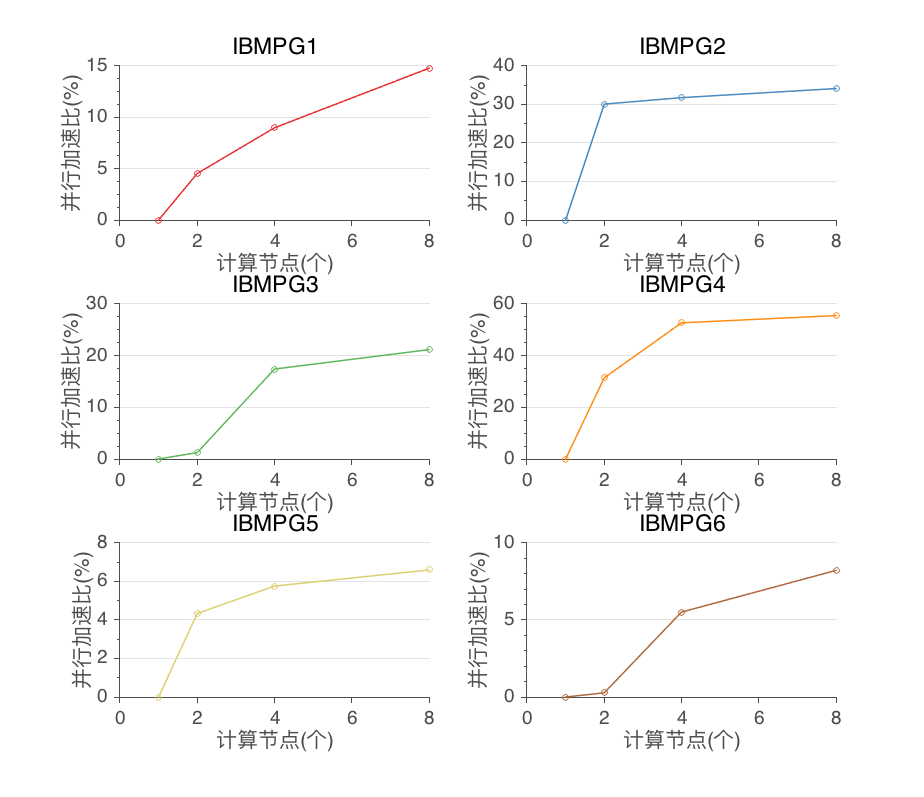
\includegraphics[height=13cm]{comm-all-ver}
  \caption{通讯量与计算节点数的关系}
  \label{fig:figcomm}
\end{figure}

\section{本章小结}

本章通过对IBM的供电网络数据集的实验,证明了第三章中提出的算法的正确性与有效性。其中,并行化对程序的效率提升起到了关键的作用:随着进程数
/使用的核心数的增加,共轭梯度算法中的各种基本运算操作都得到了有效的并行加速,从而使得程序的效率呈近线性增加;虽然在进程间通讯方面有一定的开销,
但效率的提升仍然显著。除了并行化,多重网格预条件子也对算法的效率提高起到很重要的作用,增加了收敛的速度,大大减少了迭代的次数。
